The proposed method presented in this section involves two main processes:
learning from a source task and adapting to a new target task.
The main objective is to build an agent that can perform consistently well on both source and target tasks.
In order to achieve this,
the general of this novel idea
is to allow the agent to repeatedly review the knowledge learned from the source task,
while learning the new knowledge of the target task.
The idea is inspired by a human learning effect, which is repetition learning.
Prior studies in neuroscience have proved that when humans learn by repetition,
their memory performance can be enhanced and retained for a longer time \cite{Memory_Effect_1, Memory_Repetition_1, Memory_Repetition_2},
giving humans the unique ability to perform most sophisticated tasks with ease.
Therefore,
developing a similarly intelligent method is focused on in order to achieve the main research objective and to tackle the task adaptation problem in imitation learning.


Accordingly,
the proposed method is two-fold.
Firstly,
an adaptation algorithm is proposed to allow the agent to learn the new target task by expanding its knowledge.
More concretely,
on top of the knowledge that the agent has learned from a source task,
the knowledge of a target task is added.
In addition,
the agent repeatedly uses such knowledge to learn the target task and review the previously learned source task to ensure that the learning performance on the target task is high,
while the deterioration of
the learning performance on the source task is small.
Secondly,
to support the expansion of the to-be-learned knowledge,
a novel imitation learning (IL) agent is proposed.
This agent encodes the learned knowledge into a
latent space, namely task embedding space,
in which the learned knowledge from task $x$ at time step $t$ can be represented by a high-dimensional vector $z^t_x \in \mathbb{R}^n$.
Figure \ref{ch:DTAIL:fig:TaskEmbeddingSpace} illustrates the task embedding space before and after applying the proposed task adaptation algorithm.
The task embedding space allows the proposed adaptation algorithm to add the new knowledge of the target task while minimizing its impacts on the source task's knowledge.
In addition,
since the source and target tasks are related to each other,
there are some common knowledge between those two tasks.
This shared common knowledge can be captured by the task embedding that helps accelerate the adaptation process.
The details of the proposed method are provided in the following sub-sections.

\begin{figure}[htbp!]
  \centering
  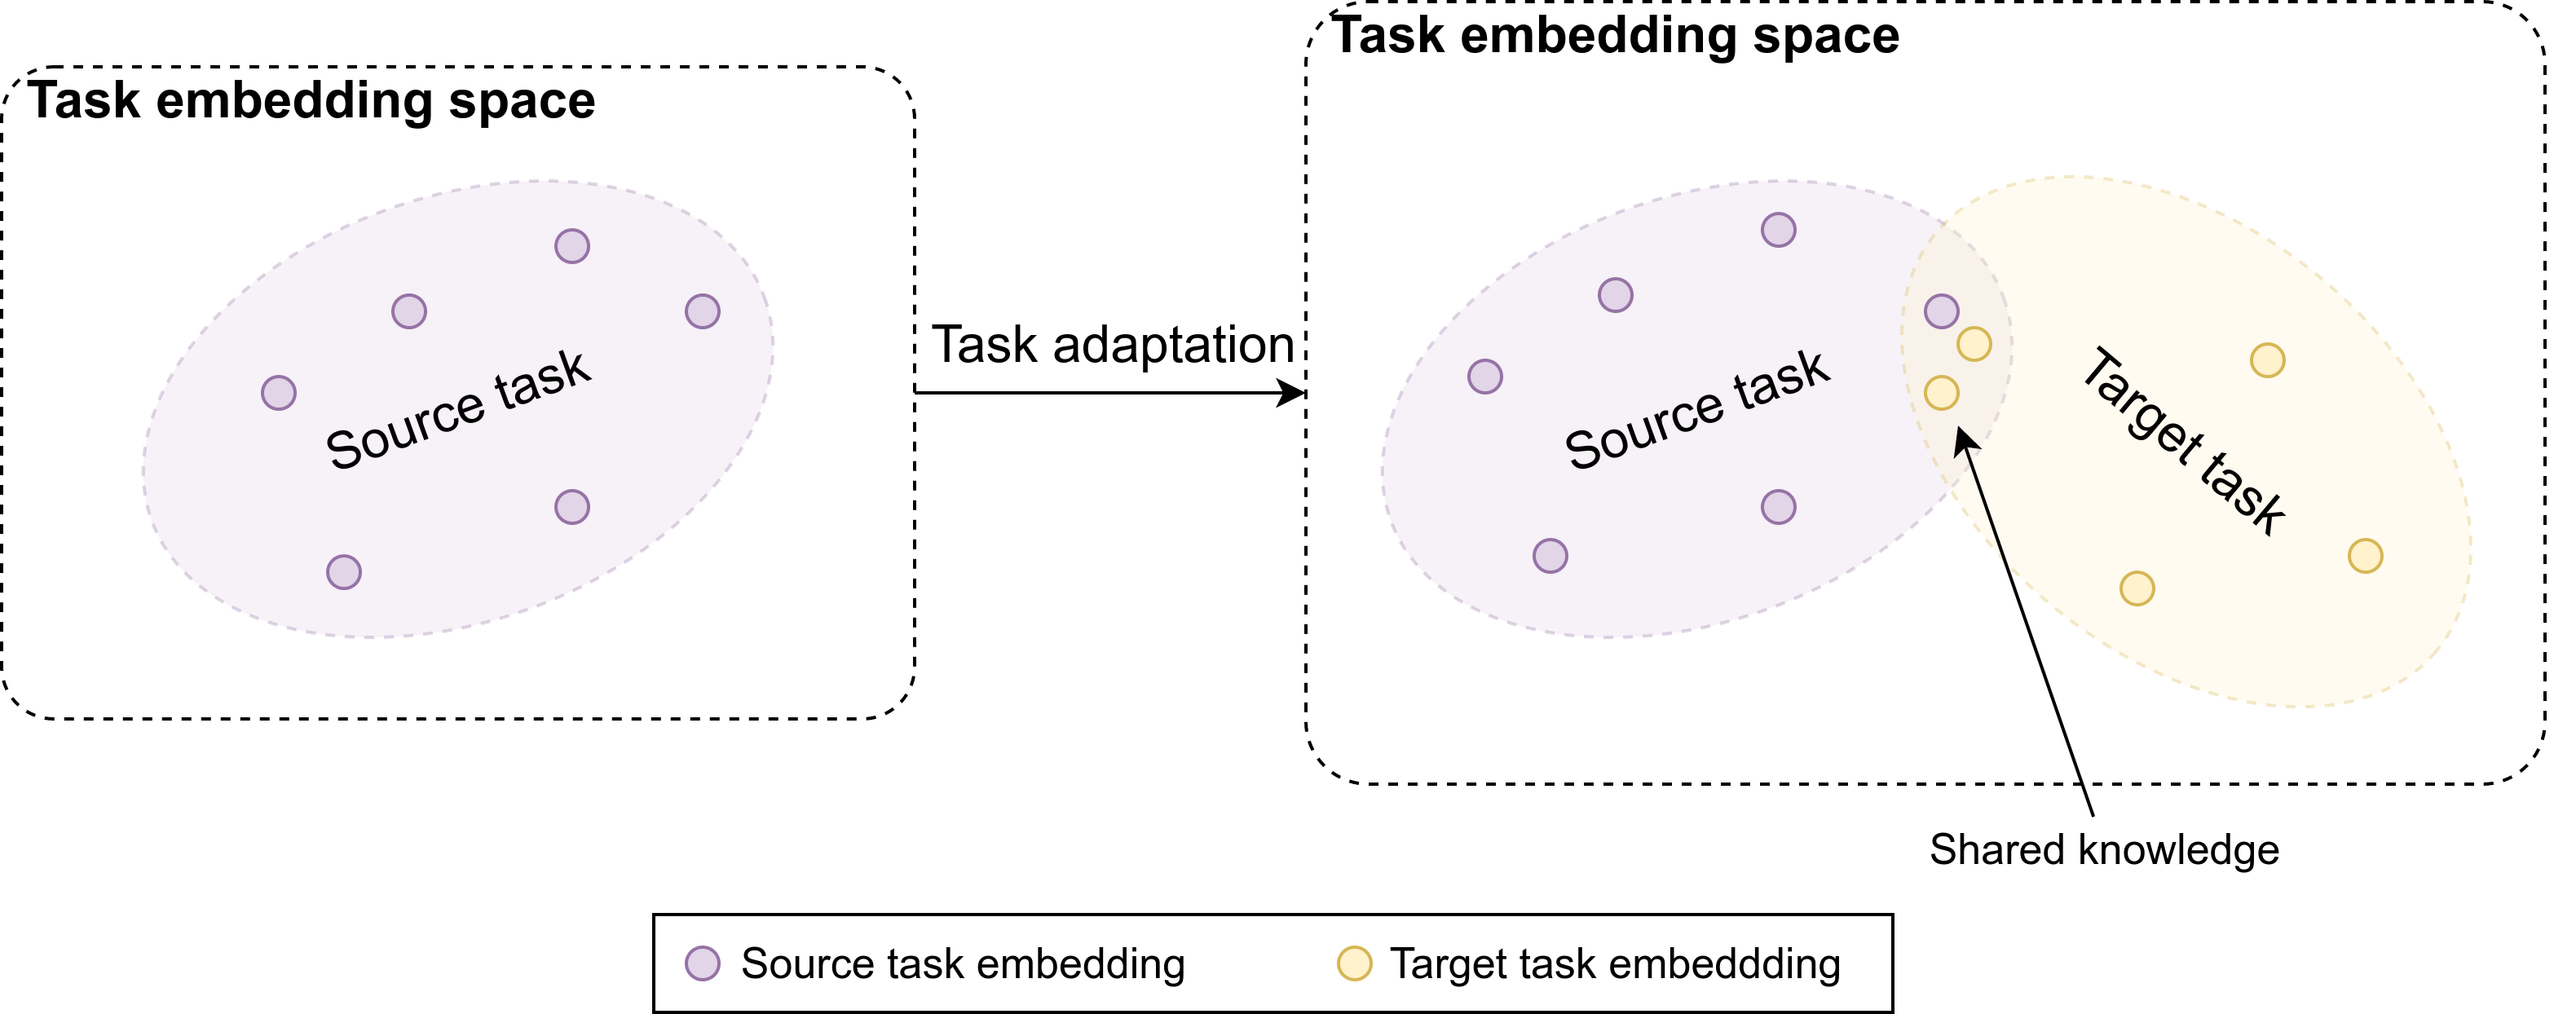
\includegraphics[width=0.9\textwidth]{\FigsDir/TaskEmbeddingSpace.png}
  \caption{An illustration of the task embedding space. Purple and yellow regions denote the knowledge learned from the source and target tasks, respectively. Applying the proposed task adaptation algorithm will lead to the expansion of the task embedding space due to the acquisition of the knowledge of the target task. In addition, the intersection between those two regions indicates the shared common knowledge between the two tasks.}
  \label{ch:DTAIL:fig:TaskEmbeddingSpace}
\end{figure}
\unskip


\subsection{The Proposed \DTAIL{} Agent}
In this subsection, the proposed agent is described in detail.
The proposed agent is an imitation learning method that finds an optimal policy for the source task using expert-generated demonstration data.
The agent is capable of encoding the learned knowledge into a task embedding in order to support the later adaptation progress.
The architecture of the proposed agent is illustrated in Figure \ref{ch:DTAIL:fig:Architecture}.
The proposed agent is a combination of three deep feed-forward networks $E$, $G$, and $D$, which have different responsibilities.


\begin{figure}[htbp!]
  \centering
  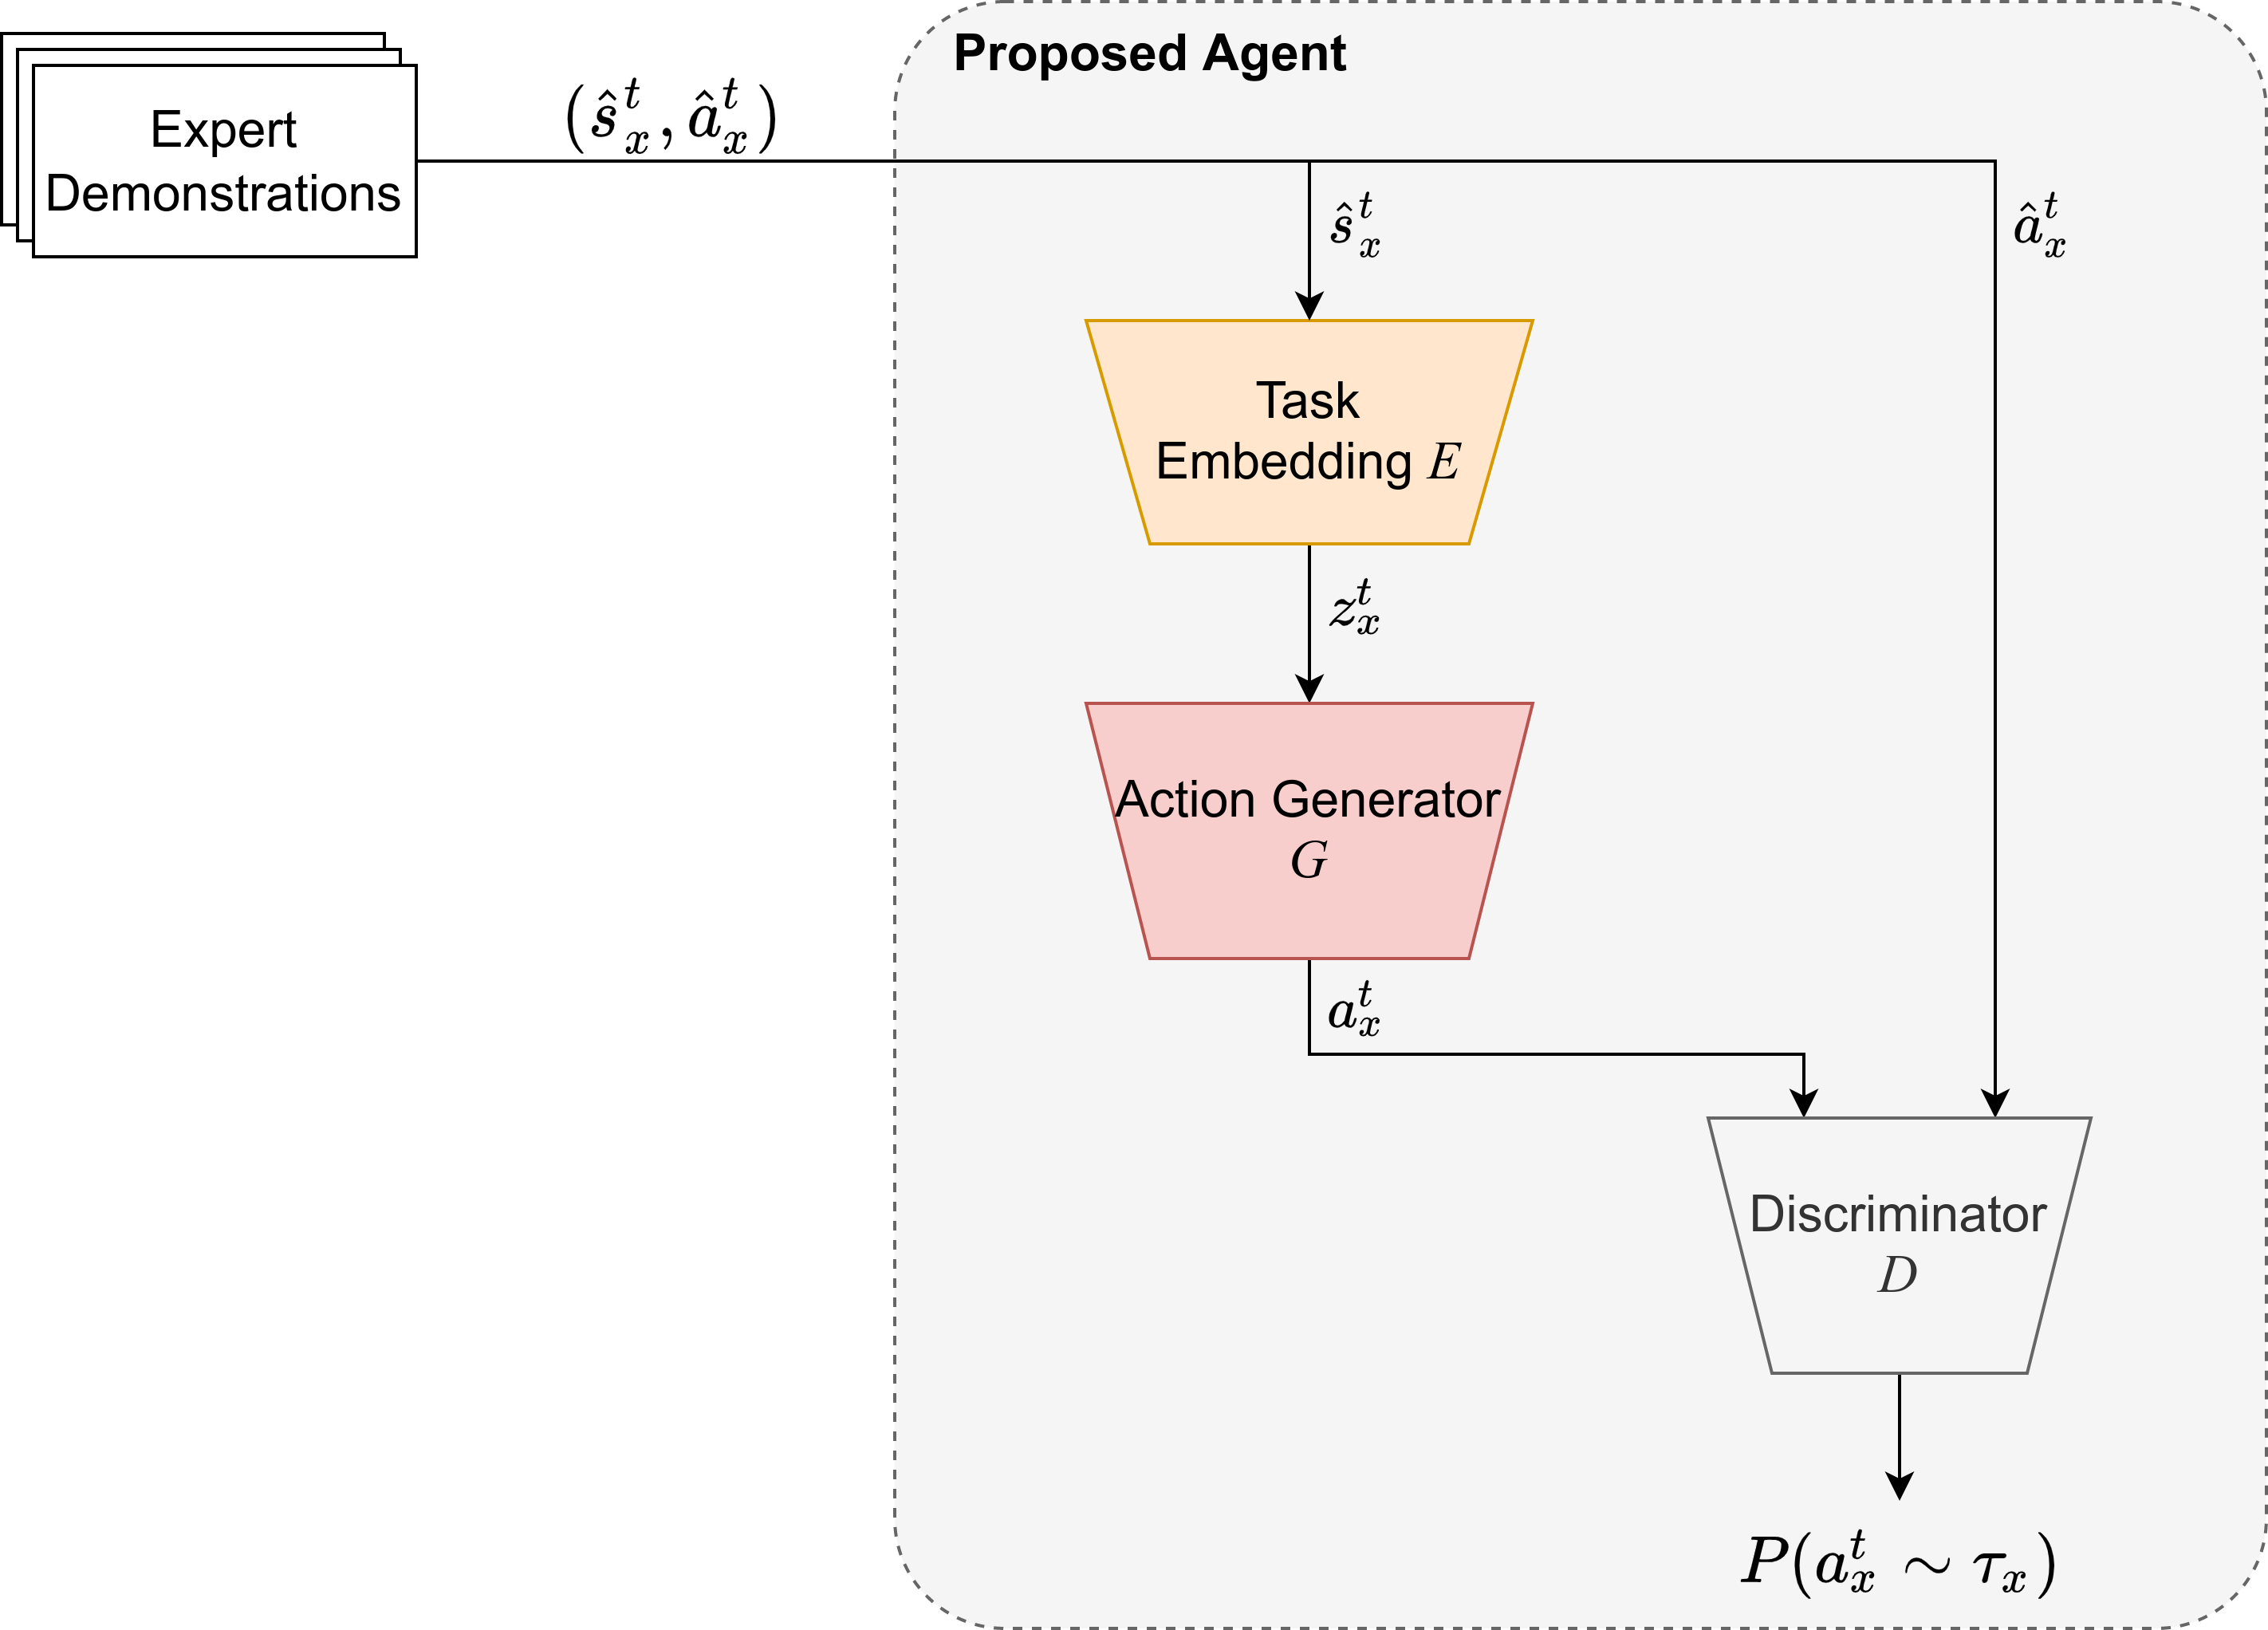
\includegraphics[width=0.9\linewidth]{\FigsDir/ModelArchitecture.png}
  \caption{The neural network architecture of the proposed agent.}
  \label{ch:DTAIL:fig:Architecture}
\end{figure}
\unskip


\subsubsection{Task-Embedding Network $E$}


The task-embedding network $E$ is designed to encode the learned knowledge into a high-dimensional task embedding space.
Specifically,
$E$ maps a state $s^t_x$ of task $x$ at time step $t$ into a task embedding $z^t_x = E(s^t_x)$, $z^t_x \in \mathbb{R}^n$.
Since $z^t_x$ contains the information of the task,
it is expected that $z^t_x$ can capture the similarities and differences between source and target tasks.
In order to achieve that,
contrastive learning is introduced to train $E$.
Contrastive learning aims to bring task embeddings of the same task close to each other in the task embedding space and to push dissimilar ones far apart.
In order words,
$E$ is trained to minimize distance $d(z^t_S, z^t_S)$ and maximize distance $d(z^t_S, z^t_T)$, where $d(\cdot)$ is a negative cosine similarity function defined as
\begin{equation}
  d(z^t_x, z^t_y) = - \frac{z^t_x \cdot z^t_y}{||z^t_x|| * ||z^t_y||}
\end{equation}
where $x$ and $y$ can be the same or different task.


The optimization function $\mathcal{L}_E$ to train $E$ is defined as follows:
\begin{equation}
  \min_{E}{\mathcal{L}_{E}(z^t_x, z^t_y) =
  \mathbbm{1}[x = y]d(z^t_x, z^t_y)
  + \mathbbm{1}[x \neq y](-d(z^t_x, z^t_y))
  }
\end{equation}
where $\mathbbm{1}(\cdot) \in \{0, 1\}$ is an indicator function.


\subsubsection{Action Generator Network $G$ and Discriminator Network $D$}

The action generator network $G$ aims to generate an optimal action $a^t_x$ using the input task embedding $z^t_x$.
The discriminator network $D$ is designed to distinguish between expert action $\hat{a}^t_x$ and the training agent's action $a^t_x$.
The intuition behind this is that the expert actions are assumed to be optimal in the imitation learning setting,
thus,
$G$ are trained to minimize the difference between $\hat{a}^t_x$ and $a^t_x$.
In order to achieve that,
the adversarial loss \cite{IL_Model_GAIL} is applied for both networks:
\begin{equation}
  \min_{G} \max_{D} \mathcal{L}_{GD}(\hat{a}^t_x, a^t_x) = \mathbb{E}[log D(a^t_x)] + \mathbb{E}[log (1 - D(\hat{a}^t_x))]
\end{equation}

The optimal policy is achieved using a RL-based policy gradient method,
which relies on reward signal $r=-log D(\hat{a}^t_x)$ provided by the discriminator.


\subsubsection{Full Objective}

During the source task's learning process,
a set of expert-generated demonstrations $\{ \tau^1_S, \tau^2_S,... \}$ is provided where each demonstration is a sequence of state-actions pairs $\tau^i_S = \{ (\hat{s}^t_S, \hat{a}^t_S),... \}$.
The task embedding for each demonstration state $z^t_S$ at time step $t$ can be computed using $z^t_S = E(\hat{s}^t_S)$.
It should be noted that the contrastive loss function $\mathcal{L}_E$ used to train $E$ requires two inputs $z^t_x$ and $z^t_y$, where $x$ and $y$ can be of the same or different task.
In this source task learning process,
the target task demonstrations are not provided yet,
thus,
the second task embedding input $z^{\prime t}_S$ is generated by introducing the Gaussian noise $\mu$$\sim$$\mathcal{N}(0, 1)$ to augment $\hat{s}^t_x$ as follows:
    \begin{equation}
      z^{\prime t}_S = E(\hat{s}^{\prime t}_S)
    \end{equation}
    where $\hat{s}^{\prime t}_S = \hat{s}^t_S + \mu$.
    In addition,
    since $\hat{s}^{\prime t}_S$ is an augmentation of $\hat{s}^t_S$,
    it might not belong to the state space $\mathcal{S}_S$ of the source task.
    Thus,
    the resulting $z^{\prime  t}_S$ is not used as an input to $G$ to generate an action, but it is used to help compute the loss $\mathcal{L}_E$ only.
    This means that $z^{\prime  t}_S$ can be treated as a constant.
    In other words,
    the gradient flows back from $z^{\prime  t}_S$ is unnecessary in the backpropagation.
    This can be indicated using the stop-gradient operation $stopgrad(\cdot)$ as follows \cite{CL_Stopgrad_1, CL_Stopgrad_2}:
    \begin{equation}
      z^{\prime t}_S = stopgrad(E(\hat{s}^{\prime t}_S))
    \end{equation}


    With the generated action $a^t_S = G(z^t_S)$,
    the full objective function to train the proposed agent on the source task is
    \begin{equation}
      \min_{E, G}\max_{D}\mathcal{L} = \mathcal{L}_E(z^t_S, z^{\prime t}_S) + \mathcal{L}_{GD}(\hat{a}^t_S, a^t_S)
    \end{equation}

    The algorithm to train the proposed agent on the source task is outlined in Algorithm \ref{ch:DTAIL:algo:Training}.


    \begin{algorithm}[H]
      \caption{Training the proposed agent on the source task.\label{ch:DTAIL:algo:Training}}
      \begin{algorithmic}[1]
        \Input
        \Desc{$\{ \tau^1_S, \tau^2_S,... \}$}{A set of expert demonstrations on the source task}
        \EndInput

        \State Randomly initialize task embedding network $E$, generator $G$ and discriminator $D$
        \For {k = 0, 1, 2, ...}
        \State Sample an expert demonstration $\tau^i_S$
        \State Sample state-action pairs $(\hat{s}^t_S, \hat{a}^t_S)$$\sim$$\tau^i_S$

            \State Compute $z^t_S = E(\hat{s}^t_S)$
            \State Compute $z^{\prime t}_S = stopgrad(E(\hat{s}^t_S + \mu))$
            \State Generate action $a^t_S = G(z^t_S)$
            \State Compute the loss $\mathcal{L} = \mathcal{L}_E(z^t_S, z^{\prime t}_S) + \mathcal{L}_{GD}(\hat{a}^t_S, a^t_S)$
            \State Update the parameters of $F$, $G$, and $D$
            \State Update policy $\pi_{S}$ with the reward signal $r=-logD(\hat{a}^t_S)$
        \EndFor

        \Output
        \Desc{$\pi_{S}$}{Learned policy for source task}
        \EndOutput
      \end{algorithmic}
    \end{algorithm}



    \subsection{The Proposed Task Adaptation Algorithm}
    Leveraging the task embedding space learned by the proposed agent,
    a novel adaptation algorithm is presented in order to adapt the agent to a new target task by adding the knowledge of the target task to the task-embedding space as shown in Figure \ref{ch:DTAIL:algo:TaskAdaptation}.
    In addition,
    to prevent losing the previously learned knowledge to perform the source task,
    a novel idea based on repetition learning is applied in the proposed adaptation algorithm.
    The idea can be illustrated as shown in Figure \ref{ch:DTAIL:fig:LearningExperience}.
    The intuition behind this idea is that during the adaptation process,
    the agent is allowed to repeatedly review how to perform the previously learned source task while learning the target task.
    Each time the agent switches to a different task,
    its performance drops,
    but then it recovers.
    This distinctive learning process allows the agent to continuously review its learned knowledge and generalize to both source and target tasks, resulting in an agent that can perform well on both tasks.
    It is similar to humans;
    when humans repeatedly practice an action,
    it leads to better performance.
    In addition,
    the process enables the agent to surpass the performance of an agent that is adapted using transfer learning.
    As shown in Figure \ref{ch:DTAIL:fig:LearningExperience},
    using transfer learning,
    the adapted agent completes its adaptation process right after adapting the source task to the target task.
    For this reason,
    when facing the source task again after adaptation,
    the performance of the agent deteriorates due to the catastrophic forgetting problem.


    It is important to note that,
    theoretically,
    the more knowledge the agent gains,
    the higher performance the agent can provide on both source and target tasks.
    As shown in Figure \ref{ch:DTAIL:fig:LearningExperience},
    after facing the source task again,
    the performance of the agent on the source task increases.
    However,
    in practice,
    there is still an amount of performance deterioration on the source task since the agent is not able to fully utilize the learned knowledge.
    This observation is further discussed in the evaluation and discussion sections.


    A hyperparameter $\lambda \in [0, 1]$ is introduced, which denotes the probability that the agent repeatedly reviews the source task's knowledge.
    With $\lambda$,
    the balance between the performance on the target task and the performance deterioration on the source task can be controlled.
    For instance,
    the higher the value of $\lambda$,
    the higher the probability that the agent can review the previously learned source task,
    resulting in a smaller deterioration of the source task's performance in exchange for low performance on the target task.
    It should be noted that if $\lambda \approx 0$,
the proposed task adaptation algorithm can be seen as a transfer learning method where it is only focused on improving the target task's performance.
The task adaptation algorithm is outlined in Algorithm \ref{ch:DTAIL:algo:TaskAdaptation}.



\begin{figure}[htbp!]
  \centering
  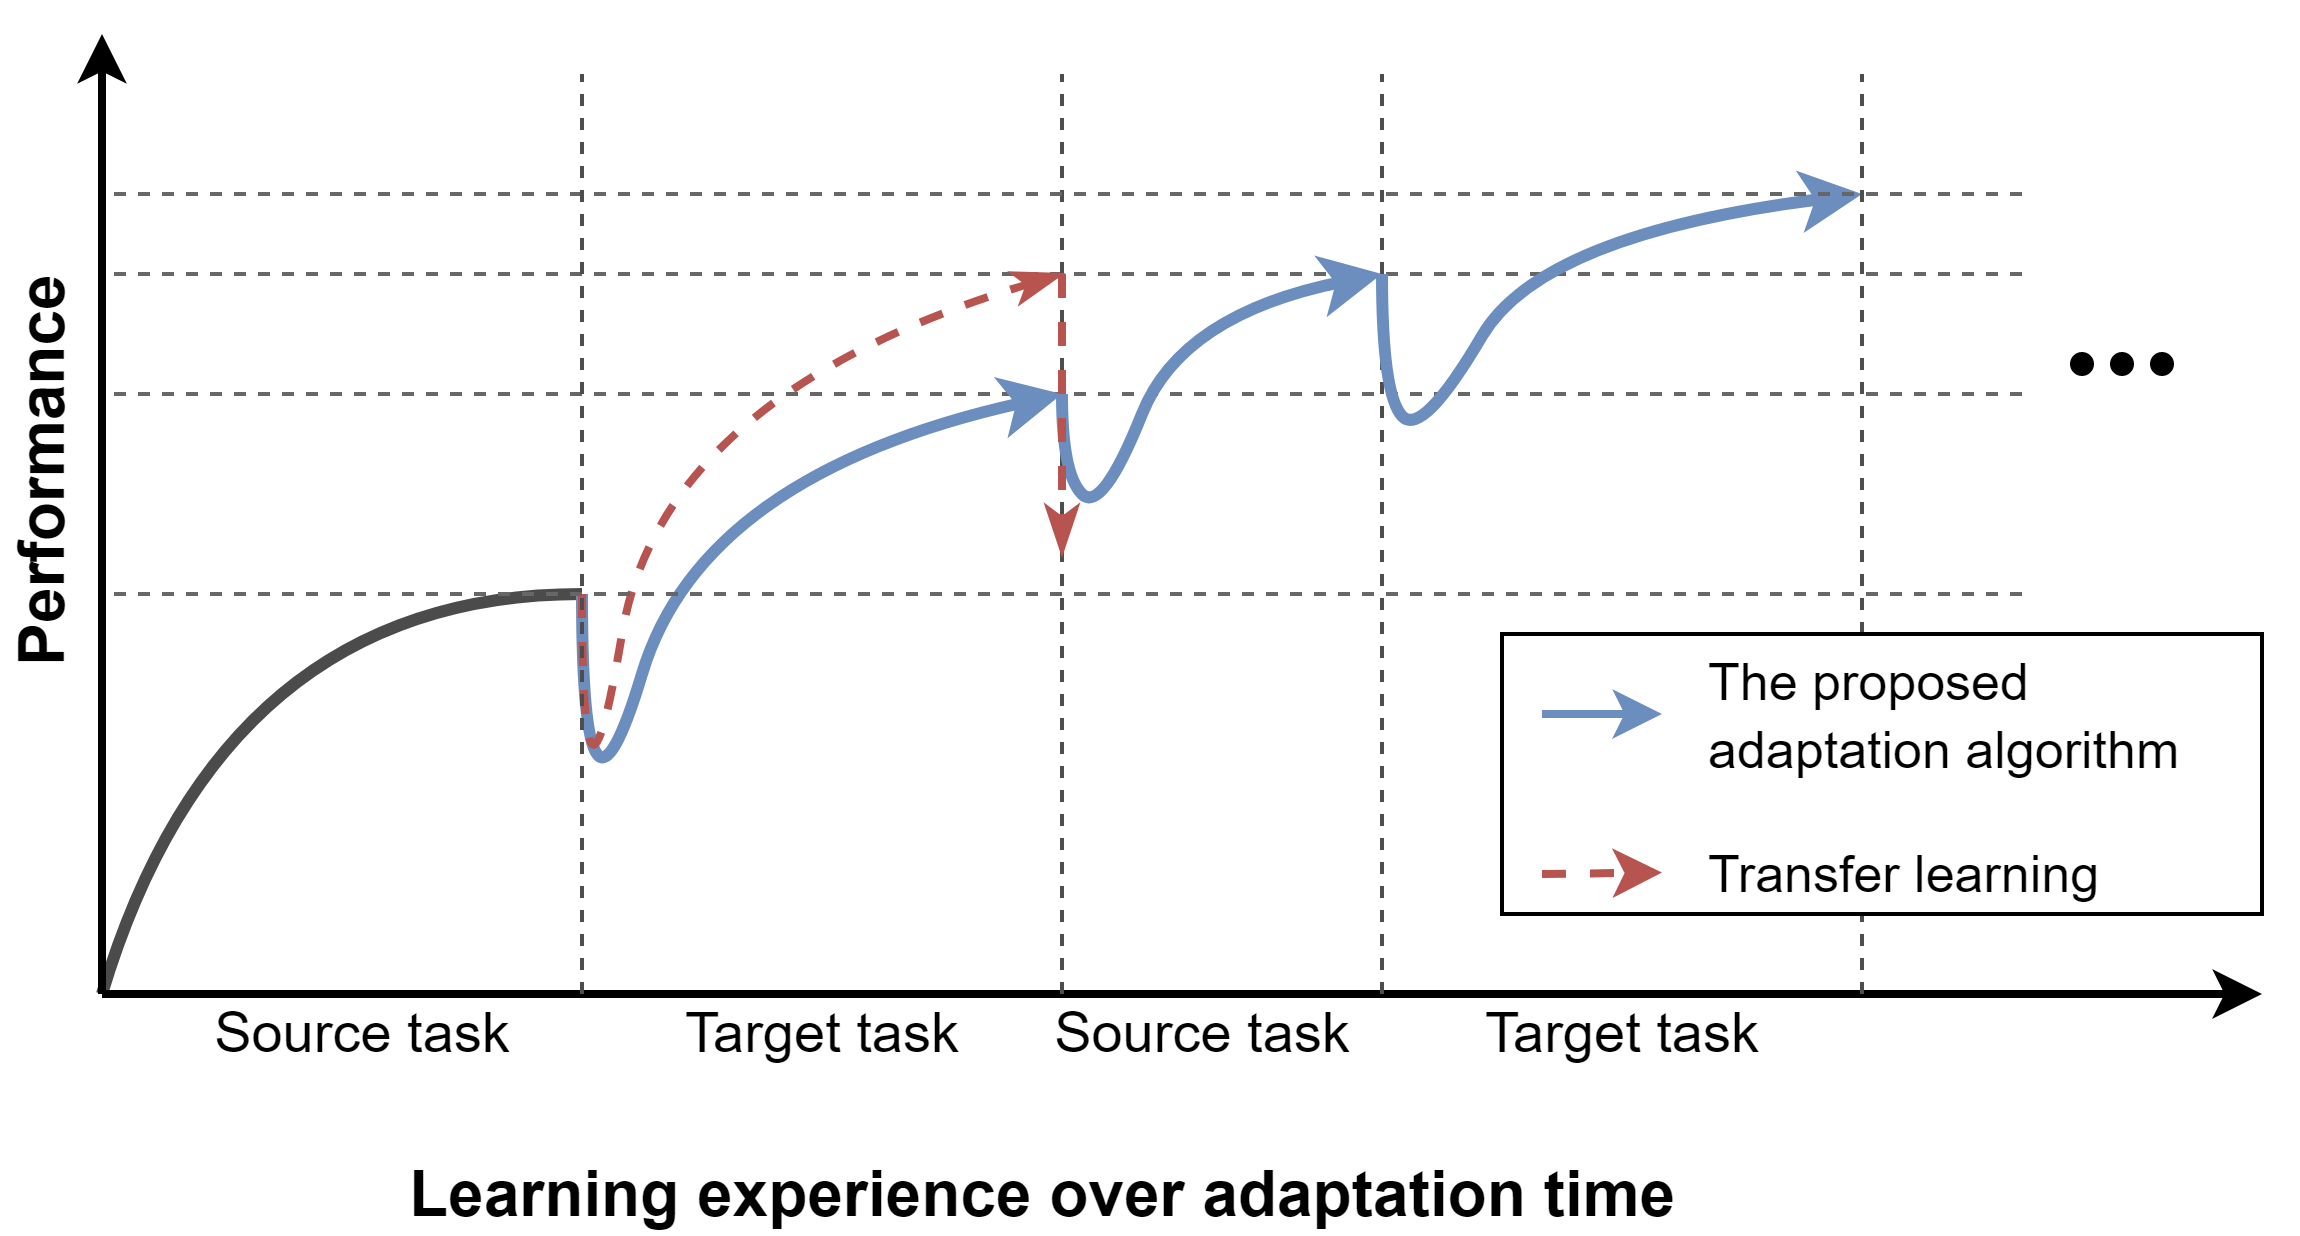
\includegraphics[width=0.8\linewidth]{\FigsDir/LearningExperience.png}
  \caption{An illustration of the performance of an agent on the source and target tasks over \mbox{adaptation time}.\label{ch:DTAIL:fig:LearningExperience}}
\end{figure}

\begin{algorithm}[H]
  \caption{The proposed adaptation algorithm.\label{ch:DTAIL:algo:TaskAdaptation}}
  \begin{algorithmic}[1]
    \Input
    \Desc{$\{ \tau^1_T, \tau^2_T,... \}$}{A set of expert demonstrations on the target task}
    \Desc{$\{ \tau^1_S, \tau^2_S,... \}$}{A set of expert demonstrations on the source task}
    \EndInput

    \State Randomly initialize task embedding network $E$, generator $G$ and discriminator $D$
    \For {k = 0, 1, 2, ...}
    \State Sample an expert demonstration on the target task $\tau^i_T$
    \State Sample an expert demonstration on the source task $\tau^i_S$
    \State Sample state-action pairs $(\hat{s}^t_S, \hat{a}^t_S)$$\sim$$\tau^i_S$ and $(\hat{s}^t_T, \hat{a}^t_T)$$\sim$$\tau^i_T$
        \State $n$ $\leftarrow$ uniform random number between 0 and 1

        \If {$n < \lambda$}
        %\Then
        \Comment{Review source task's learned knowledge}
        \State Compute $z^t_S = E(\hat{s}^t_S)$
        \State Compute $z^t_T = stopgrad(E(\hat{s}^t_T))$
        \State Generate action $a^t_S = G(z^t_S)$
        \State Compute the loss $\mathcal{L} = \mathcal{L}_E(z^t_S, z^t_T) + \mathcal{L}_{GD}(\hat{a}^t_S, a^t_S)$
        \Else
        \Comment{Learn target task}
        \State Compute $z^t_T = E(\hat{s}^t_T)$
        \State Compute $z^t_S = stopgrad(E(\hat{s}^t_S))$
        \State Generate action $a^t_T = G(z^t_T)$
        \State Compute the loss $\mathcal{L} = \mathcal{L}_E(z^t_T, z^t_S) + \mathcal{L}_{GD}(\hat{a}^t_T, a^t_T)$
        \EndIf
        \State Update the parameters of $F$, $G$, and $D$
        \State Update policy $\pi_{S}$ with the reward signal $r=-logD(\hat{a}^t_S)$
    \EndFor

    \Output
    \Desc{$\pi_{ST}$}{Learned policy for both source and target task}
    \EndOutput
  \end{algorithmic}
\end{algorithm}
